%%%%%%%%%%%%%%%%%%%%%%%%%%%%%%%%%%%%%%%%%%%%%%%%%%%%%%%%%%%%%%%%%%%%%%%%%%%%%%%%%%
%%% Navigation Control
%%%
%%%
%%%%%%%%%%%%%%%%%%%%%%%%%%%%%%%%%%%%%%%%%%%%%%%%%%%%%%%%%%%%%%%%%%%%%%%%%%%%%%%%%%
\chapter{Perception and Navigation}
\label{ch::navigation}


	\section{Flatland navigation and goal (feature) tracking}
	
		The BlueFoot robot is operated using a potential field-based control scheme for obstacle avoidance during navigation over flatland. Camera-based feature tracking has been incorporated into this navigation scheme for the purpose of establishing goals to which the robot attempts to travel to. Platform navigation is administered by two main command parameters, $v^{r}$ and $\omega^{r}$, which represent forward velocity and turning rate of the platform with respect to the robot's trunk frame $O_{b}$. During navigation, the pitch of the trunk, $\theta_{b,x}$ is also controlled via its respective reference signal, $\theta_{b,x}^{r}$. Control over trunk pose allows for additional articulation of the LIDAR and camera sensors mounted to BlueFoot's head (trunk). 

		Namely, BlueFoot's potential fields-based navigation mechanism fuses LIDAR data and features from processed camera images. This algorithm is essentially used as a ``wandering" mechanism which would normally be employed as a first-level navigation measure in an unknown environment when no information (\IE environmental map data) is known by the robot \emph{a priori}. Camera features are used in conjunction with LIDAR scans for the purpose of assigning trackable targets, which are a particularly useful in navigation for avoid local minima faced with navigating via a potential-fields approach, alone. Moreover, image features as points of attraction, which draw the robot towards them. 

		This section will first describe the base potential-fields algorithm, which utilizes only LIDAR sensor data. Results related to this navigation mechanism will be presented from simulation. Then, the incorporation of processed camera data will be described and a set of associated results will be presented from real-world trials.

		\subsection{LIDAR-based Potential-Fields Algorithm}

			The LIDAR-base portion of this algorithm takes  planar LIDAR scans as an input and generates a set of navigation outputs, $\vec{u}^{r}_{L} \in \Re^{3}$, which represents a direction of travel relative to the world frame, $O_{0}$, and $P_{L}$, which represents a total positive potential . Each point from a LIDAR scan is mapped to a corresponding scalar \emph{potential} which is used to influence the direction of the newly generated command. Given a LIDAR scan, $S^{L}$, with 2D scan points, $x_{i}^{L}\in\emph{S}^{L}$, relative to the LIDAR's local coordinate frame $O_{L}$, an output command vector is generated using a potential function $\{ f(x) : \Re^{3}\rightarrow \Re^{1} \}$, and a biasing function, $\{ g(x,\psi) : \Re^{3}\rightarrow \Re^{1} \}$, as follows:
				\begin{eqnarray}
				%x_{i}  &=& P_{ \vec{z} } \wrap{ H_{b}^{0} H_{L}^{b} \Gamma_{L} x_{i}^{L} } \nonumber\\
				%\bar{x}_{b,i} &=&  x_{i}-p_{b} \nonumber \\
				\vec{u}^{r}_{L} &=&  { \sum_{x_{i}^{L} \in \emph{S}} g( x_{i}^{L},\psi)  f( x_{i}^{L} ) \frac{x_{i}^{L}}{\norm{x_{i}^{L}}} } \nonumber \\
				P_{L} & = & \alpha_{p}\sum_{x_{i}^{L} \in \emph{S}^{L}} g( x_{i}^{L},\psi)  f( x_{i}^{L} ) U\wrap{f( x_{i}^{L} )}
				\end{eqnarray}
			%where $H_{b}^{0}$ defines a homogeneous transformation between $O_{0}$ and $O_{b}$; $H_{L}^{b}$ defines a homogeneous transformation which relates the LIDAR's pose to the frame $O_{b}$; $\emph{S}\subset \Re^{3}$ is the set of newly transformed points, $x_{i}^{L} \in \emph{S}$, relative to the current LIDAR scan in the world coordinate system; 
			%where $U(*)$ is the standard unit-step function;  $\alpha_{p}$ is a scalar tuning parameter; and 
			%	\begin{equation*}
			%		\Gamma_{L} = \sbrack{ I_{2\times2}, 0_{2\times1} }^{T}.
			%	\end{equation*}
			%Since we are assuming navigation over flat ground, the operator $P_{ \vec{z} }\wrap{*}$ is used to project each transformed LIDAR scan-point's onto the plane defined by the unit vector pointing in the unit-vector direction of the $z$-axis in the frame $O_{0}$.

			The piecewise potential function, defined in \ref{eq::min_dis_potential_function}, is used in BlueFoot's navigation scheme, This function is designed to ``repel" the platform from objects which are closer to the robot than some minimum distance, $d_{min}$, and ``attract" the robot toward objects that are further away. The form of this potential function was guided by several candidate force-field functions presented in \cite{ArambulaCosio2004}. The intention of \ref{eq::min_dis_potential_function} is to draw the robot towards long apertures, such as corridors or openings, and away from close-by obstructions. It is written as follows:
				\begin{eqnarray}
					\Delta d &\equiv& \norm{x}-d_{min} \nonumber \\
					f(x) &=& 
					\begin{cases}	
					 	 -\lambda_{c,1} \wrap{\Delta d}^{2} &  \text{if } \Delta d < 0 \\
						\wrap{\Delta d} \wrap{ 1  - e^{ -  \lambda_{c,2} { \wrap{\Delta d} }^{2} } } 	&  \text{else}
					\end{cases}
				\label{eq::min_dis_potential_function}
				\end{eqnarray}
			where $\lambda_{c,1}>0$ and $\lambda_{c,2}>0$ are tuning parameters used to specify the output range and sensitivity of the potential function output with respect to $\Delta d$, respectively. It can be observed that this potential function exhibits $f(x)<0$ when $\norm{x} < d_{min}$ and vice-verse, thus achieves the desired attractive and repulsive characteristics. Namely, this potential function favors points which are generally much further away from the robot, and applies \emph{strong} repulsive forces only when obstacles come within a close range with the platform. These characteristics offer a higher propensity for exploration when the area being navigated is very spacious with few obstacles in view (but at mid range), while encouraging \emph{tight} navigation around from potential obstacles. A visualization of  the potential field, $f(x)$ is shown in Figure \ref{fig::potential_field} for a $2$-by-$2$ meter area about the robot. Note the negative potential values about the obstacles, which result in repulsive forces.
				\begin{figure}[t!]
					\centering
					\fbox{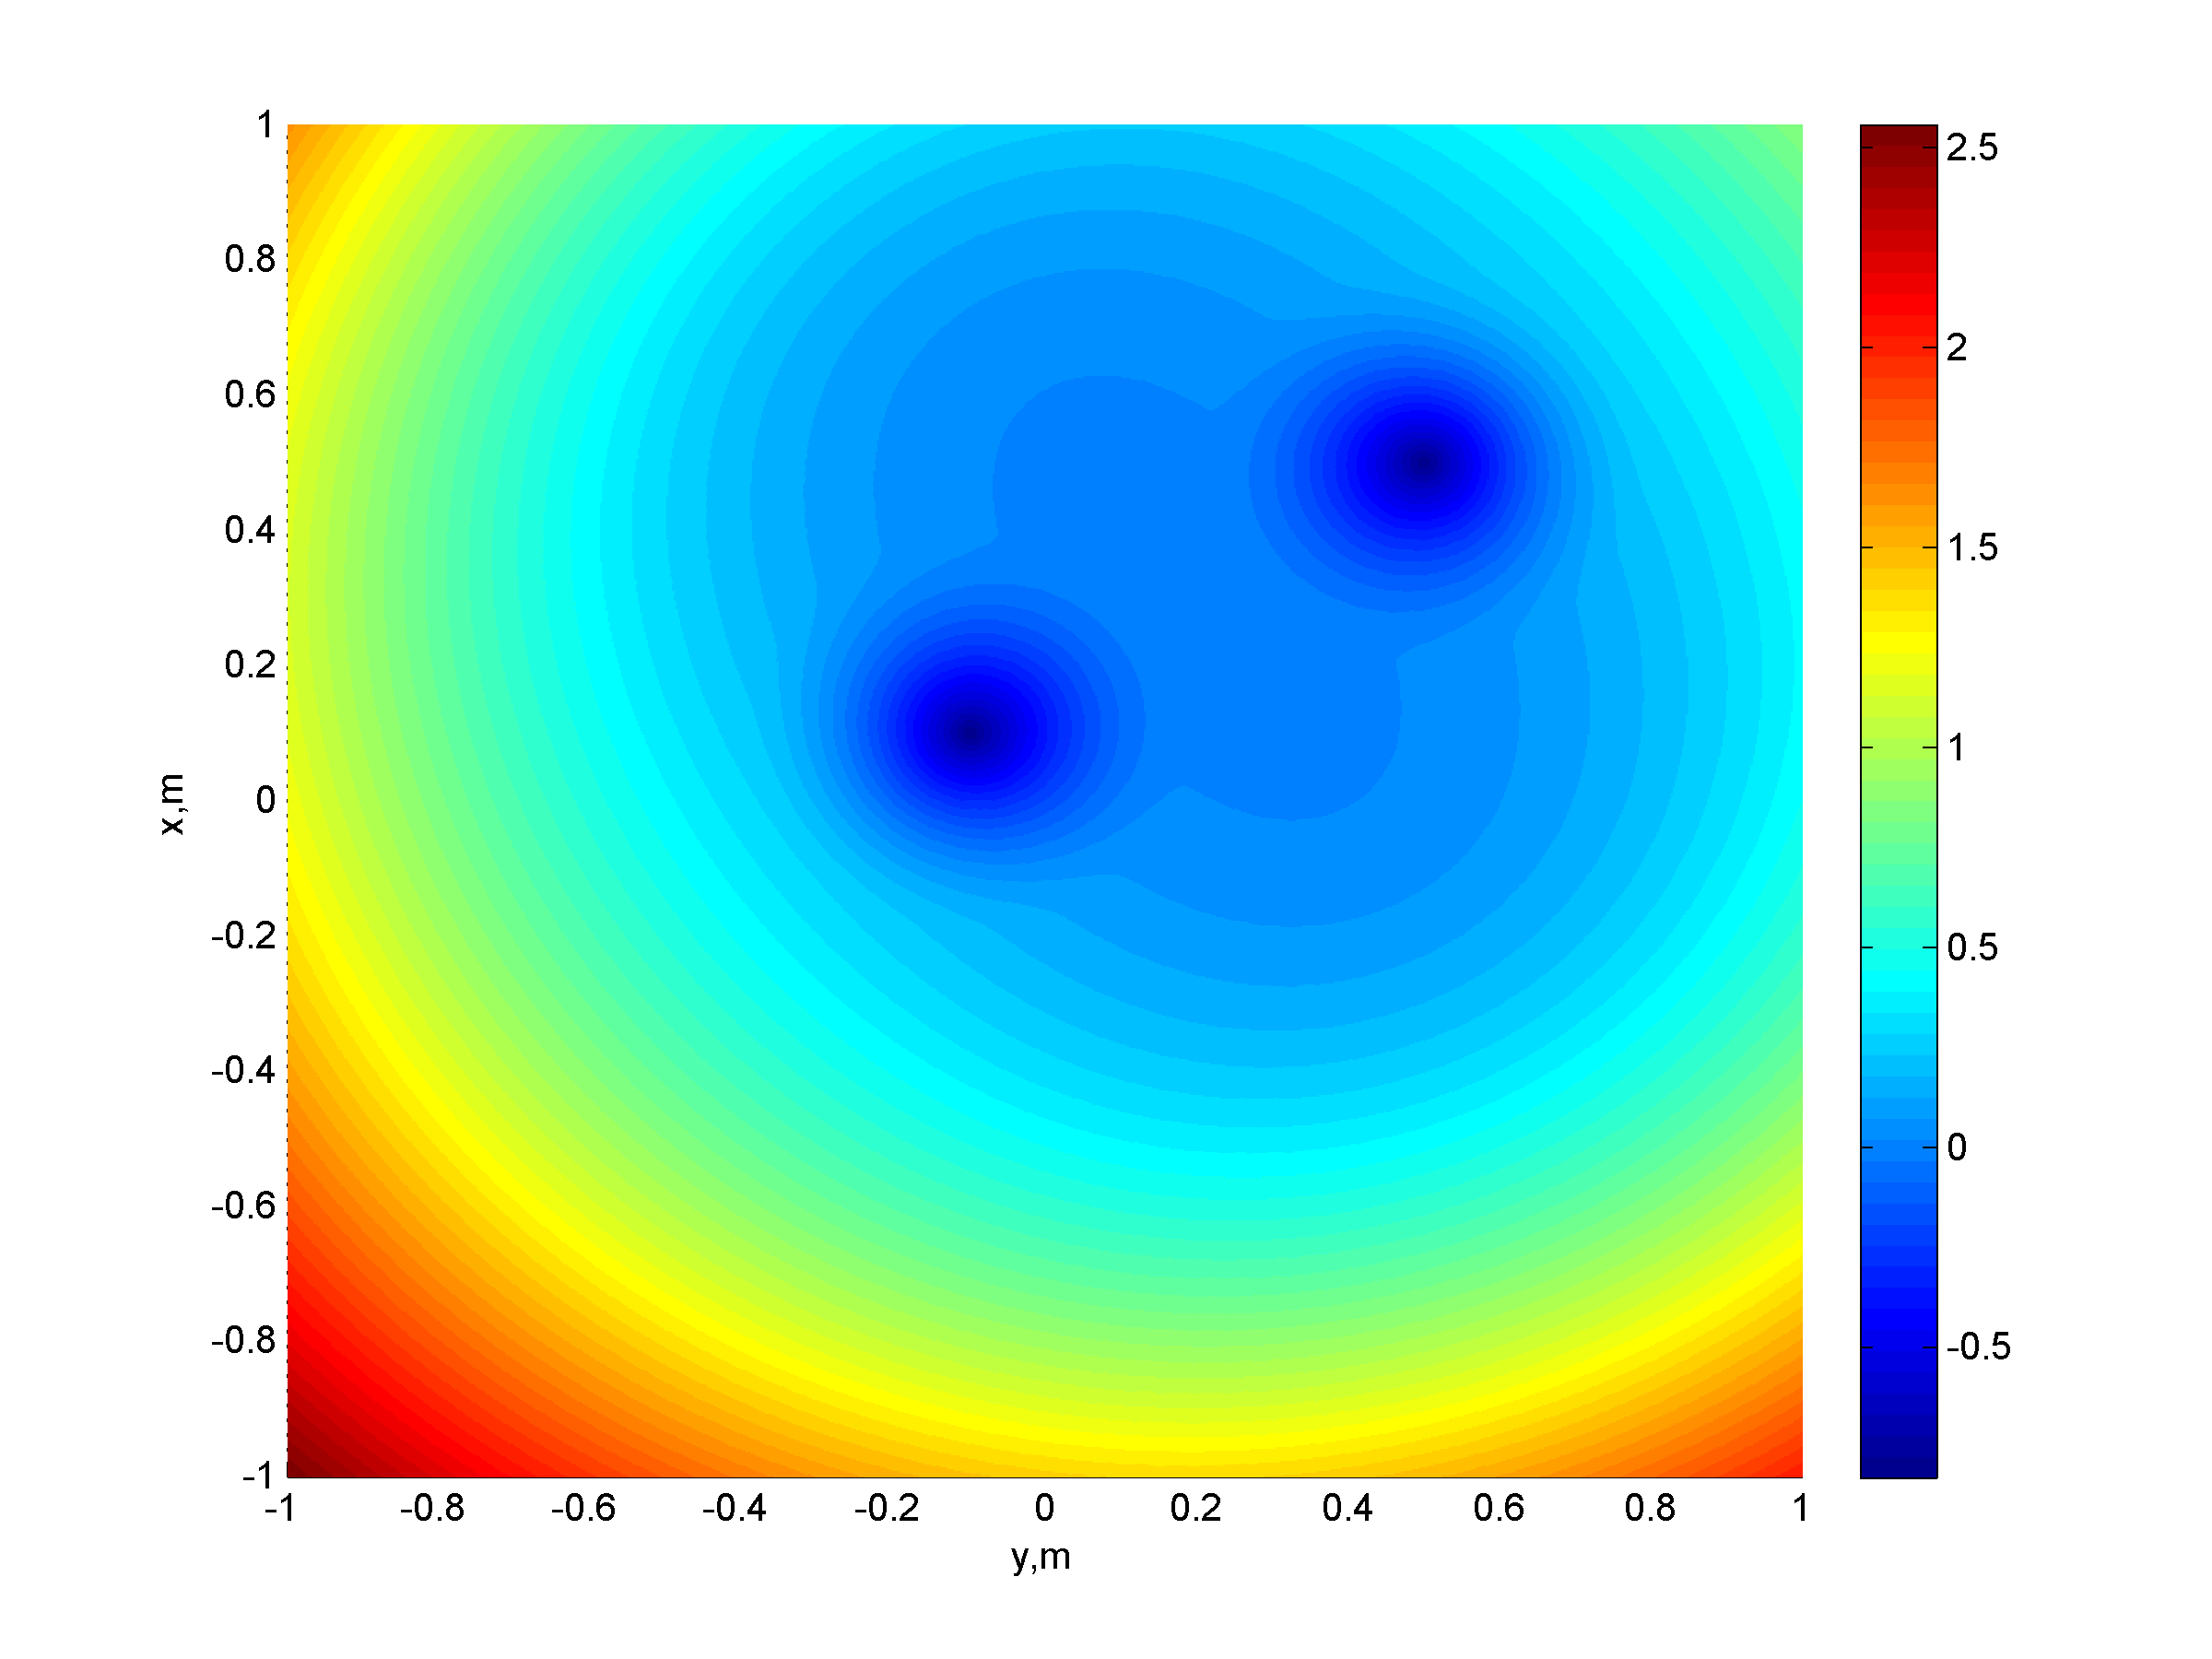
\includegraphics[width=\textwidth]{potential_field.png}}
					\caption{Potential field, $f(x)$ with $d_{min}=0.4m$ given an environment with with obstacles. Objects are located at $(0.5,0.1)\text{ m}$ and $(0.1,-0.1)\text{ m}$ from the robot. }
					\label{fig::potential_field}
				\end{figure}

			The biasing function $g(x,\psi)$ is used to weight the effect of individual points from a single scan on the final output, with respect to their relative angular position. The biasing function is parametrized with an angular-window parameter $\psi>0$. A simple masking-type biasing function is used in BlueFoot's navigation function, which is formally defined as follows:
				\begin{eqnarray}
					\text{ang}\wrap{x} &=& \tan^{-1}\wrap{ \frac{\xcomp{x}}{\ycomp{x}} } \nonumber\\
					g(x,\psi) &=& 
					\begin{cases}
					\wrap{1-\abs{\frac{\text{ang}\wrap{x}}{\psi}}}^{\alpha}	& \text{ang}\wrap{x} < \psi \\
					0 	& \text{otherwise}.
					\end{cases}
				\end{eqnarray}
			where $\xcomp{x}$ and $\ycomp{x}$ are the $x$-axis and $y$-axis coordinates of the vector argument $x\in\Re^{3}$; and $\alpha\leq1$ such that . This function is used to give priority points which exists in a front-ward facing angular window, spanning $2 \psi$, centered at the $y$-axis which emenates from $O_{L}$. Considering only frontward points serves to reduce the potential for getting stuck in local minima, namely when the robot moves into an area where it faces equal potential from all sides. 
			%In the event that the robot does get stuck in a potential minima, a ``stuck" detection algorithm has been implemented. As the name suggests, this algorithm first detects if the robot is stuck in a local minima of the potential field based on a window of command histories.

			Finally, outputs of the potential field algorithm are transformed into forward and turning rate commands, ${v}_{L}^{r}$ and $\omega_{L}^{r}$, respectively, by the following proportional control scheme:
				\begin{eqnarray}
					\theta_{L}^{r} 			&=& \tan^{-1}\wrap{ \frac{ \xcomp{\vec{u}^{r}_{L}} }{ \ycomp{\vec{u}^{r}_{L}} } } \nonumber\\
					\dot{v}_{L}^{r} 		&=& \beta_{v} \wrap{ P_{L} + v_{L,min}^{r} - v_{L}^{r} } \nonumber \\
					\dot{\omega}_{L}^{r} 	&=& \beta_{\omega} \wrap{ \wrap{ \frac{ \omega_{L}^{r,max} }{\pi} } \wrap{  \theta_{L}^{r} - \theta_{b,z} } - \omega_{L}^{r} }
				\end{eqnarray}
			where $\beta_{v}$ and $\beta_{\omega}$ are proportional-gain tuning parameters; $v_{L,min}^{r}>0$ is a small, minimum velocity used to prevent the robot from getting stuck in local minima; and $\theta_{b,z}$ is robot's yaw in $O_{0}$. The parameters $\beta_{v}$ and $\beta_{\omega}$ can be viewed as ``update-inertias," as they directly effect the influence of the effect of instantaneous commands on the forward velocity and turning rate of the robot. Furthermore, these gains can be used to low-pass updates to navigation parameters so as to remove jitter cause by potential outliers generated from degenerate sensor readings.


		\subsection{Simulated potential field navigation results}

				\begin{figure}[h!]
					\centering
					\fbox{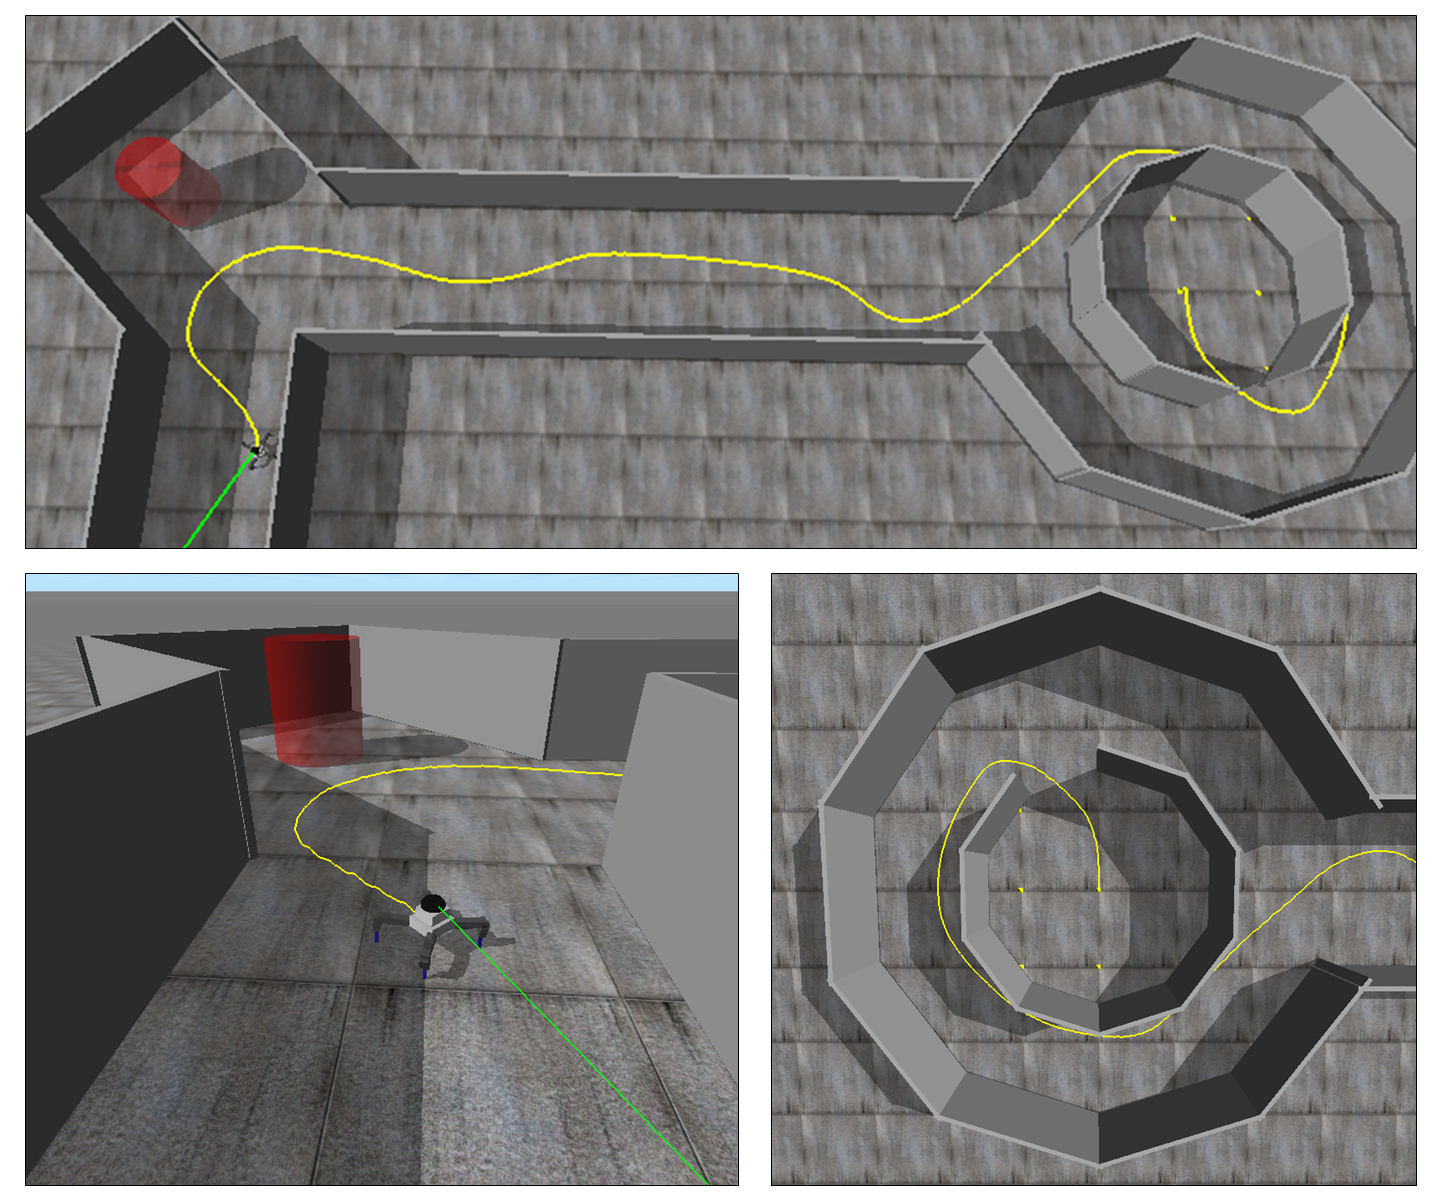
\includegraphics[width=\textwidth]{potential_field_full.png}}
					\caption{Path (shown in yellow) taken by robot through a simulated set of rooms and halls using the LIDAR-based potential fields navigation scheme.}
					\label{fig::potential_field_results}
				\end{figure}
				\begin{figure}[h!]
					\centering
					\fbox{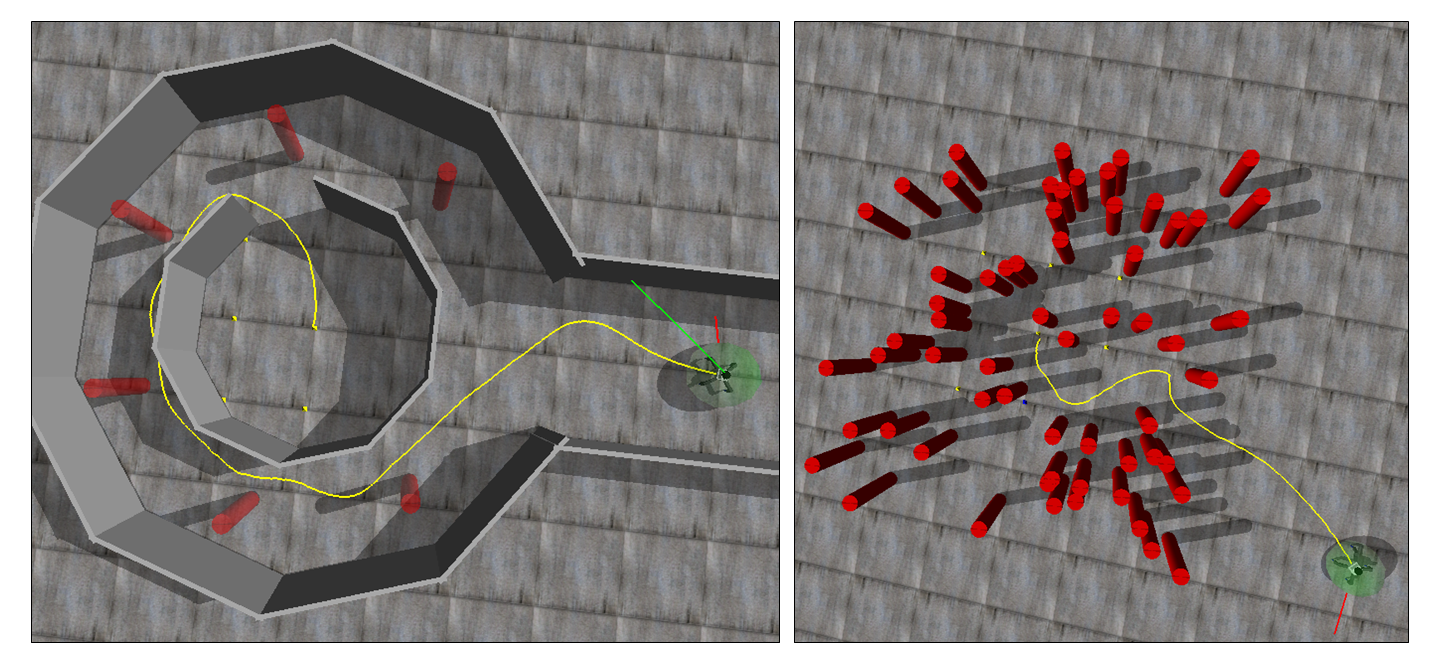
\includegraphics[width=\textwidth]{potential_field_full_obstacles.png}}
					\caption{Path (shown in yellow) taken by robot through a simulated set of rooms and obstacles.}
					\label{fig::potential_field_results_obstacles}
				\end{figure}
		
			Figure \ref{fig::potential_field_results} shows the path resulting from a simulated trial in which the BlueFoot robot autonomously wandered through an environment, consisting of a room and several long corridors. During this simulation, BlueFoot is navigated using the previously described potential-fields mechanism. A plot of the robot's trajectory (shown in yellow) shows that the robot was able to successfully navigate its immediate environment while avoiding collisions with the surrounding walls. Notably, the robot naturally avoided smaller out-cove regions, which were mostly filled with obstacles, because these regions had low relative potential. A second set of results is shown in Figure \ref{fig::potential_field_results_obstacles} shows the robot's performance in environments additional obstacles. Likewise, the robot exhibits the desired obstacle-aversion performance using the describe potential field function.


		\subsection{Incorporation of Camera-based Feature-Tracking}
		
			Camera-based goal tracking is used in conjunction with the aforementioned potential fields navigation scheme to move the platform through an environment while seeking or tracking a particular target. In this case, targets take the the form of features extracted from processed camera data. The robot is guided towards these features using a simple visual-serving approach. 

			Trackable camera features can be generated in a variety of ways. For the purpose of BlueFoot's navigation, objects with distinct shapes or color have been chosen for tracking so that shape and blob detection algorithms easily can be employed to detect the relative positions of these features in BlueFoot's viewing range. Namely, Hough Transform-based shape detection and standard color-blob detection algorithms from the Open Computer Vision (OpenCV) library are employed for the purpose of feature detection\cite{opencv_library}. Once detected, points representing the centers of each trackable feature, relative to the 2D camera-viewing frame, are mapped into forward velocity and turning rate commands. These command are used to control the robot such that the center of the feature is aligned with the center of each image fame. These camera-based commands are then mixed with the outputs of the potential-fields controller as a weighted sum to form a hybrid navigation control law.

			The visual-servoing approach to be described is agnostic of the type of feature being tracked. Namely, this approach relies on the relative position of the center of each feature, represented as a pixel-position, $p_{Im} = [u,v]^{T} \in Z^{2}$ in the 2D image frame, $O_{Im}$, and a relative size, $r$, measured in pixels. In the case of circular features, for example, $r$ represents the radius of the detected circle. For color-blob features, $r$ represents the radius of a circle which fully inscribes the colored object.

			For the purpose of target tracking, it is desired that the robot's forward speed be controlled such that is proportional to $r$. Namely, it is desired that the robot stops when it becomes \emph{close enough} to the target object, and faster towards the goal when the feature is in sight but the robot is further away. The position of the feature's center is used to control the robot's turning rate, as well as the commanded pitch of the robot's trunk, $\theta_{b,x}^{r}$. Trunk articulation important during feature tracking routing as it aids in keeping the tracked-target objects centered in the image frame. Provided that the target is moving slower than the what the system can track, this will ensure the target remains in sight at all times.

			A separate set of navigation commands, $v_{C}^{r}$ and $\omega_{C}^{r}$; and an additional body-pitching command, $\theta_{b,x}^{r}$,  are generated from an extracted feature location, $p_{Im} = [u,v]^{T}$ as follows: 
				\begin{eqnarray}
					v_{C}^{r} 			& = & v_{C}^{r,max} \wrap{ 1 - e^{ -c_{r} \wrap{ r-r_{min} }^{2} } } 	\nonumber 	\\
					\omega_{C}^{r} 	& = & \omega_{C}^{r,max} \wrap{\frac{ w_{Im} - 2 u  }{ w_{Im} } }		\nonumber 	\\
					\theta_{b,x}^{r}	& = & \theta_{b,x}^{r,max} \wrap{ \frac{ 2 v - h_{Im} }{ h_{Im} } } 		
				\end{eqnarray}
			where $v_{C}^{r,max}$, $\omega_{C}^{r,max}$ and $\theta_{b,x}^{r,max}$ are the maximum magnitude of forward velocity, turning rate, and body-pitching commands, respectively; $c_{r}$ is a sensitivity parameter; $r_{min}$ defines a minimum feature size which will result in the administration of a zero velocity command to the platform (and thus the distance from the feature at which to halt forward motion); and $w_{Im}$ and $h_{Im}$ define the width and height, respectively, of the image being processed. Having now established a formulation for how a single, distinct, feature is used to guide the platform towards a target, a means of fusing the LIDAR-based command signals and the camera-based command signals will be defined.

			The composition of this hybrid command technique is motivated by two related subtasks: 
				\begin{enumerate}
				\item to use the potential fields algorithm during a wandering phase, when a target object is not in sight and
				\item to guide the robot safely towards the goal once in sight.
				\end{enumerate}
			This causes camera-based tracking commands to have a greater influence on system navigation (through the variables $v^{r}$ and $\omega^{r}$) as the platform becomes closer to the desired target. A straight-forward way to achieve this is to use the relative size. $r$, of tracked target features in the image frame. With this in mind, a simple command mixture scheme has been defined as follows:
			\begin{eqnarray}
				v(r) &\equiv&
				\begin{cases}
				e^{ -c_{mix} \wrap{ r - r_{mix}}^{2} } 	& \text{if } r < r_{mix}	\\
				1											& \text{else}
				\end{cases}
								\nonumber \\
						\left[\begin{array}{c} v^{r} 	\\ \omega^{r} 		\end{array} \right] &=& 	
				v(r)	\left[\begin{array}{c} v^{r}_{C}\\ \omega^{r}_{C} 	\end{array} \right] + 
				(1-v(r))\left[\begin{array}{c} v^{r}_{L}\\ \omega^{r}_{L} 	\end{array} \right] 
			\end{eqnarray}
			where $c_{mix}$ is a sensitivity parameter; and $r_{mix}$ defines the processed-feature size which will cause the robot to be navigated, mostly, using camera features. The reasoning for such a scheme involves a heuristic approach to obstacle aversion, which assumes that when the platform is further away from a goal, there is a higher probability that it will encounter an obstacle. Conversely, when the goal becomes closer to the platform, it is assumed that the number of obstacles between the robot and the target is lower, making it safe to shift full priority to reaching the goal from the current position. It is defined that if a feature is not visible within the current view of the camera, then it is considered to be of size $r=0$.


	\section{Towards Rough Terrain Navigation}


		\subsection{Terrain Mapping from 2D scans}
			\label{ssec::terrain_mapping}
			\begin{figure}[h!]
				\centering
				\fbox{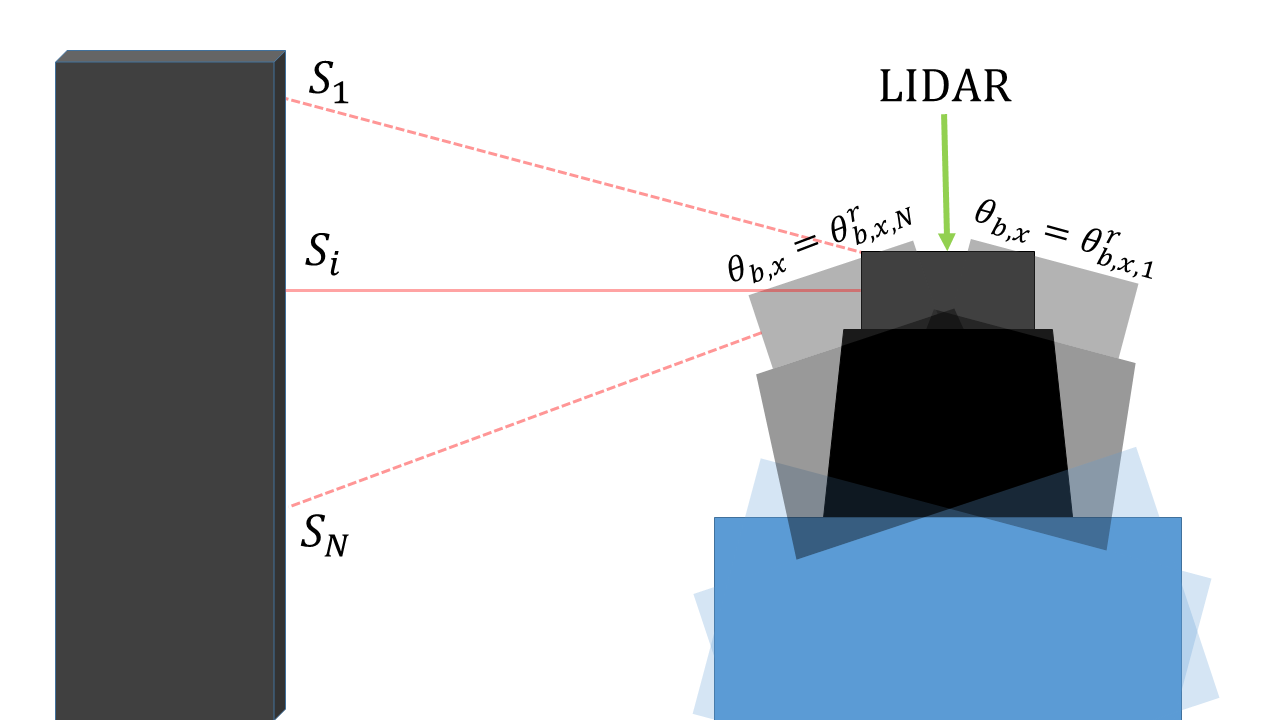
\includegraphics[width=\textwidth]{laser-sweep.png}}
				\caption{LIDAR swept over a range of angles, $\theta_{b,x} \in [\theta_{b,x,1}^{r},\theta_{b,x,N}^{r}]$. }
				\label{fig::sensor_sweep}
			\end{figure}
			The BlueFoot platform has the ability to compose 3D point clouds from a series of swept 2D LIDAR scans in conjunction with a trunk orientation estimates, $\hat{\theta}_{b}$. LIDAR articulation is achieved by slowly pitching the trunk over some angular range while keeping the platform's feet ridgedly planted. Sweeping range is limited by the kinematic-feasibility of each trunk pose that must be reached during a sweep. Given a particular set of foot and body location, kinematic feasibility is validated using the inverse kinematics solution described in Section \ref{sec::inverse_position_kinematics}. A single 2D scan is taken at each pose within the body-sweep trajectory. The newly acquired scan is transformed from the LIDAR sensor frame, $O_{L}$, to the world frame by a homogeneous transformation $H^{L}_{0}$ which is defined as follows
				\begin{equation}
					H^{L}_{0} = H^{L}_{b} H^{b}_{0}
					\label{eq::world_to_sensor}
				\end{equation}
			where $H^{b}_{0}$ is a transformation from $O_{0}$ to the trunk frame $O_{b}$, as defined in Chapter \ref{ch::system_modeling}; and $H^{L}_{b}$ defines a transformation from the frame $O_{b}$ to the LIDAR frame, $H^{L}_{b}$. $H^{L}_{b}$ is necessary for knowing the position of the LIDAR head with respect world frame, as the sensor itself has some offset and rotation relative to the robot's body. Each 2D point from $x_{i} \in \emph{S}$ from the initial scan, $\emph{S}\subset \Re^{2}$, can then be transformed into a 3D scan segment, $\bar{S}_{j}$, in $O_{0}$ by:
				\begin{equation}
					\left[
						\begin{array}{c}
							\bar{x}_{i,j} \\ 1
						\end{array}
					\right]
				 = H^{L}_{b} H^{b}_{0}	
					\left[
						\begin{array}{c}
							x_{i} \\ 0 \\ 1
						\end{array}
					\right] \forall x_{i} \in \emph{S}
					\label{eq::scan_to_segment}
				\end{equation}
			where $\bar{x}_{i,j} \in \bar{S}_{j}$ is a point withing the 3D \Jth scan segment $\bar{S}_{j} \subset \Re^{3}$. After the sweeping routine is complete, 3D scan segments are composed into a final point cloud, $\bar{S}$ by:
			\begin{equation}
				\bar{S} = \bigcup_{j=1}^{N_{s}} \bar{S}_{j}
			\end{equation}
			where $N_{s}$ defines the number of scans taken during the sweeping routine. For the sake of simplicity, it is assumed that the trunk's position, $p_{b}$, is fixed (system is completely ridged) during a swept-scan routine. In the results to be presented, this seems to be a reasonable assumption given that the platform is at rest and the trunk is pitched sufficiently slowly over the angular sweeping range. A slow sweep rate ensures that perturbations caused by vibrations incurred by trunk rotation and foot-slip are small, and thus does not cause for significant deviations in LIDAR scan points.
				\begin{figure}[h!]
					\centering
					\fbox{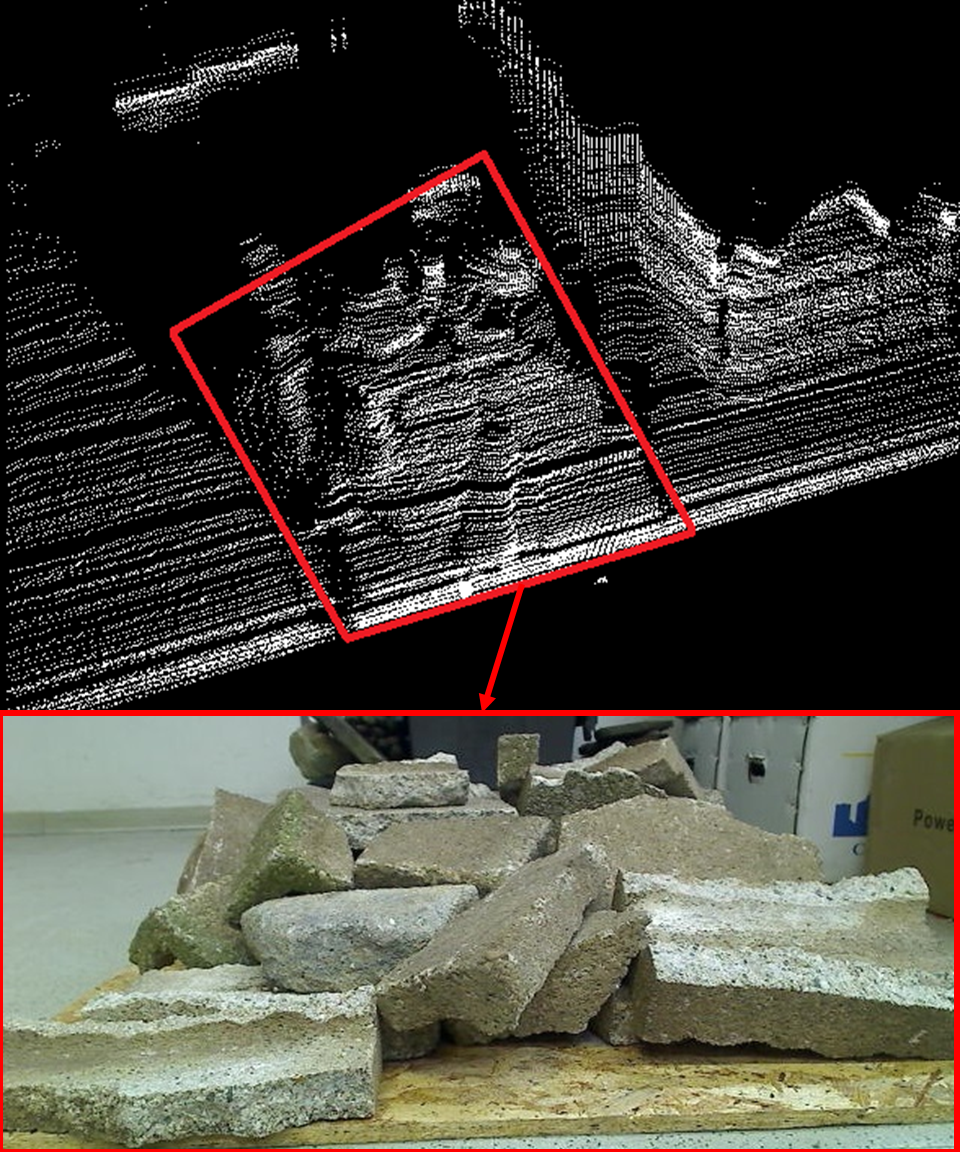
\includegraphics[width=0.95\textwidth]{rough_terrain.png}}
					\caption{Original 3D point-cloud of terrain patch \emph{(top)} and corresponding view from robot's on-board camera \emph{(bottom)}.}
					\label{fig::pointcloud_terrain_patch}
				\end{figure}


		\subsection{Height-map Generation from 3D point cloud}
			
			3D point clouds can be represented as height-maps in a fictitious height-map coordinate system, $O_{Hm}$. These representations are convenient for use in planning as they can be used to assign costs to particular robot configurations during terrain traversal straightforward way. In implementation, height-maps are generated by represented as a matrix  $M\in \Re^{n\times m}$ where the (\Ith, \Jth) indices of $M$ represent a location within the $O_{Hm}$ frame, whose height is represented by the value of the matrix element $m_{i,j}$. Essentially, point-cloud elements which exist within a $w\times d$  discretization region (region of interest) are used to build a height-map. This matrix is used as a discrete representation of point cloud points which falls within a region of interest (ROI), $\bar{S}_{ROI}\subset\Re^{3}$. The location and size of this regions would have to be determined with some auxiliary detection process first locates an appropriate ROI. Such an algorithm must perform by:
			\begin{enumerate}
				\item selecting an area with appropriately high terrain variation (large changes in gradient)
				\item and determining the bounding region where this patch of rough-terrain exists
			\end{enumerate}
			so as to generate a height-map from a subset of points in $\bar{S}$. For the results to be shown, the terrain being evaluated has been manually selected after inspection of an existing 3D point cloud, as an adequate algorithm has yet to be implemented which fulfills the requirements of the detection task described. Such an algorithm would need to involve mechanisms for point cloud segmentation and feature evaluation. Additionally, images of the the robot's immediate terrain could be used to aid in this process by locating areas with high image-feature density.

			Once an ROI is determine, the space contained the subset of point cloud elements $\bar{S}_{ROI}$ is divided into $(nm)$ sub-divisions, each of which covers a $(w/m) \times (d/n)$ area. Each (\Ith, \Jth) element of $M$, $m_{i,j}$, is then populated with the highest point (largest  $z$ component) within each  (\Ith, \Jth) subdivision. The transformation from a point cloud element $\bar{x} = [\xcomp{\bar{x}},\ycomp{\bar{x}},\zcomp{\bar{x}}]^{T}$ to an element within the discretized height-map frame, $[i,j,h]^{T} \in O_{hm}$, equivalently $m_{i,j}=h$, can be described by:
				\begin{equation}
					\left[
						\begin{array}{c}
						i \\
						j \\
						h  	\\
						\end{array}
					\right]
					=
					\ciel{
						\left[
							\begin{array}{ccc}
							n/d & 0 	& 0 \\
							0 	& m/w 	& 0 \\
							0 	& 0 	& 1 \\
							\end{array}
						\right]
						\wrap{
							\left[
								\begin{array}{ccc}
								0 &-1 & 0 \\
								1 & 0 & 0 \\
								0 & 0 & 1 \\
								\end{array}
							\right]
							\left[
								\begin{array}{c}
								\xcomp{\bar{x}} \\
								\ycomp{\bar{x}} \\
								\zcomp{\bar{x}} \\
								\end{array}
							\right]
							+
							\left[
								\begin{array}{c}
								1.5 d \\
								0.5 w \\
								0 \\
								\end{array}
							\right]
						}
					}
					\label{eq::toheightmapframe}
				\end{equation}
			where $\ciel{*}$ is an element-wise vector ceiling function. Depending on the density of the source point cloud, this height-map conversion process has the potential to produce relatively sparse height-maps. To deal with this, a dilation and smoothing routine is used to fill in gaps which exist in converted height-map. During dilation, each non-zero height element within the map is expanded into a region around an existing element with non-zero value \cite{opencv_learn_immorph}. This process is performed until a semi-uniform map is produced with minimal gaps between non-zero height elements. Finally, a median filter is applied to the dilated height-map to produce smooth transitions between height elements within the height map. The median filter replaces all values within a window of elements (usually forming a square region) with the middle-valued element.
				\begin{figure}[t!]
					\centering
					\fbox{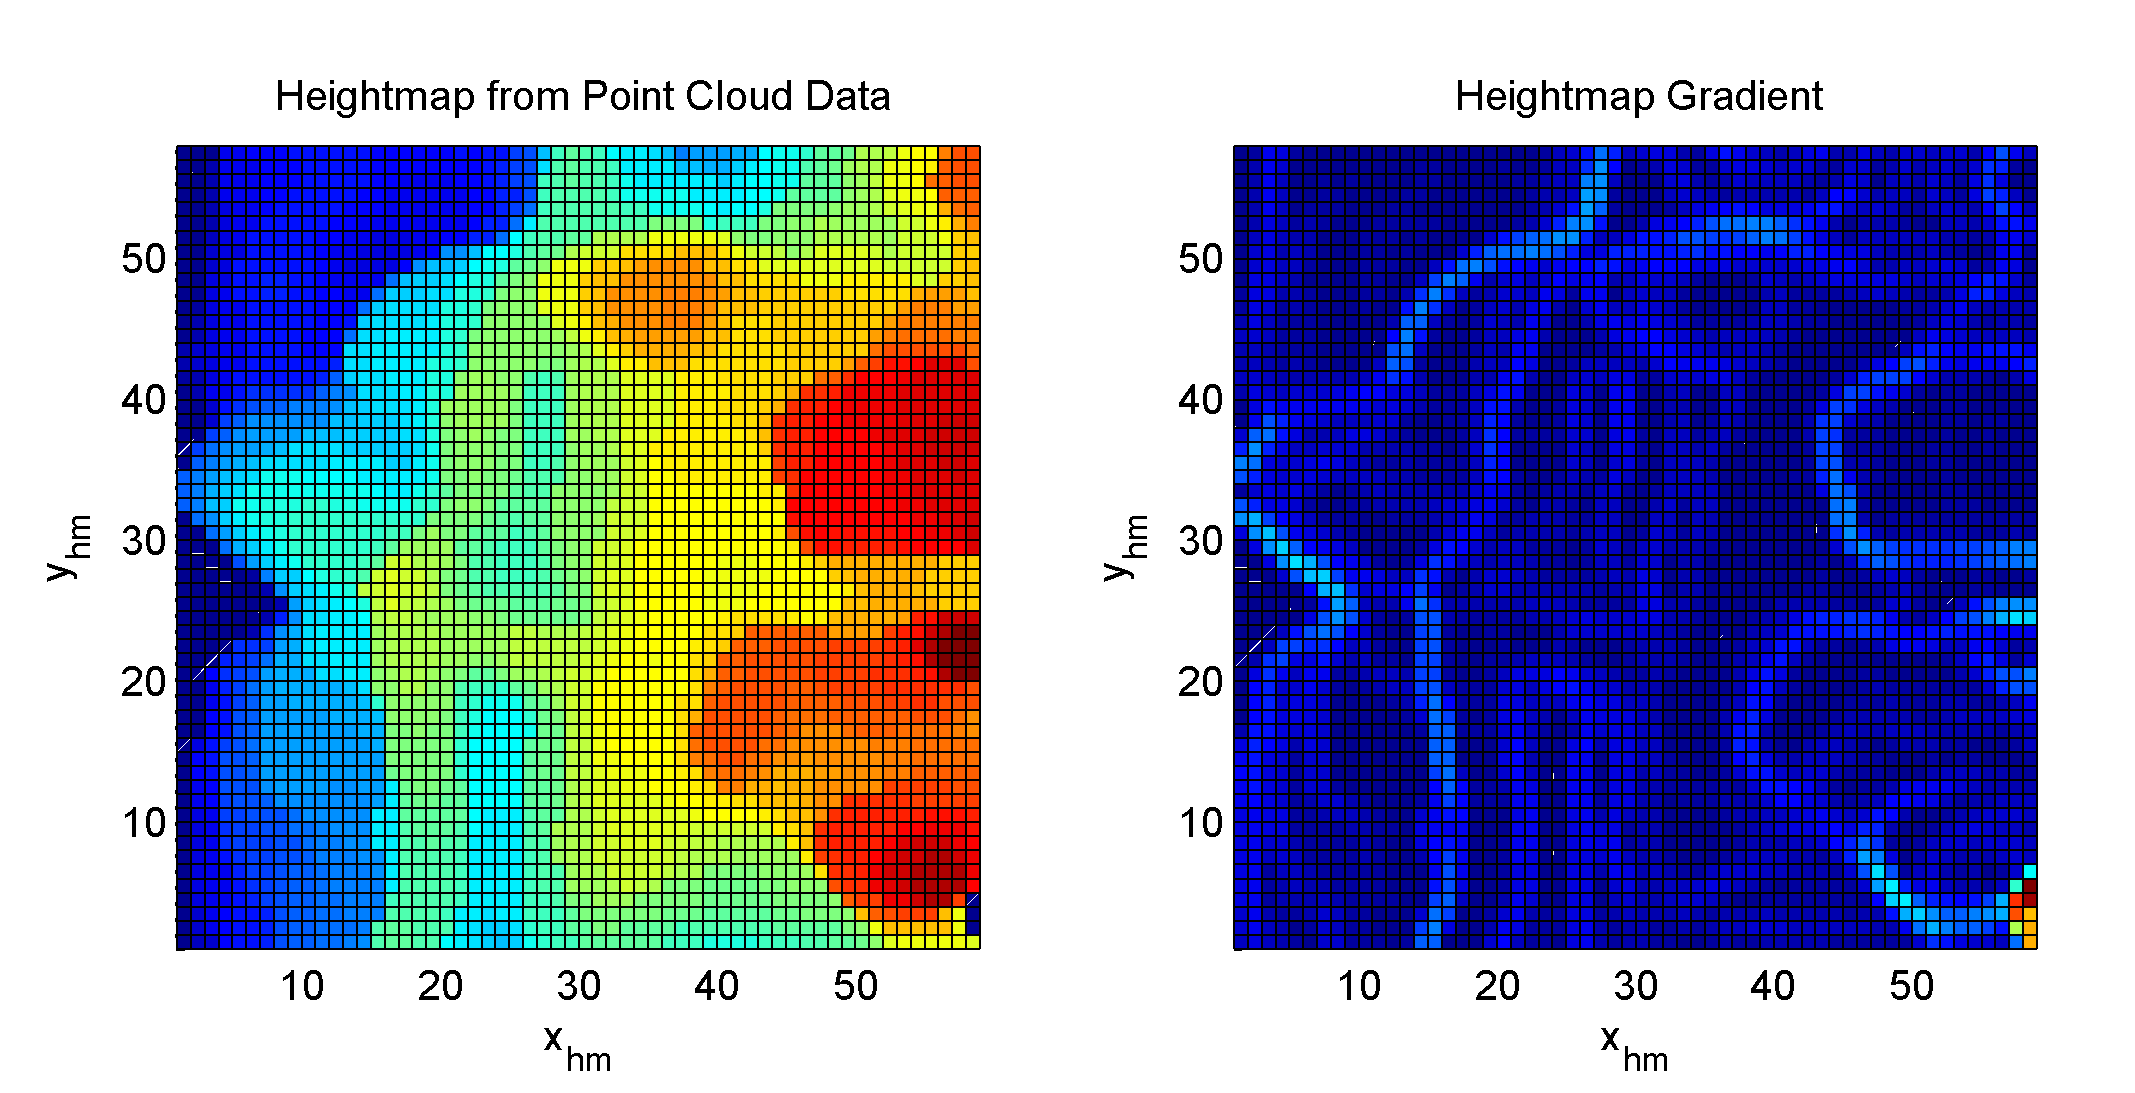
\includegraphics[width=\textwidth]{terrain_grad_crop.png}}
					\caption{Relative height-map \emph{(left)} and its corresponding gradient \emph{(right)}.}
					\label{fig::heightmap_terrain_patch}
				\end{figure}
				\begin{figure}[h!]
					\centering
					\fbox{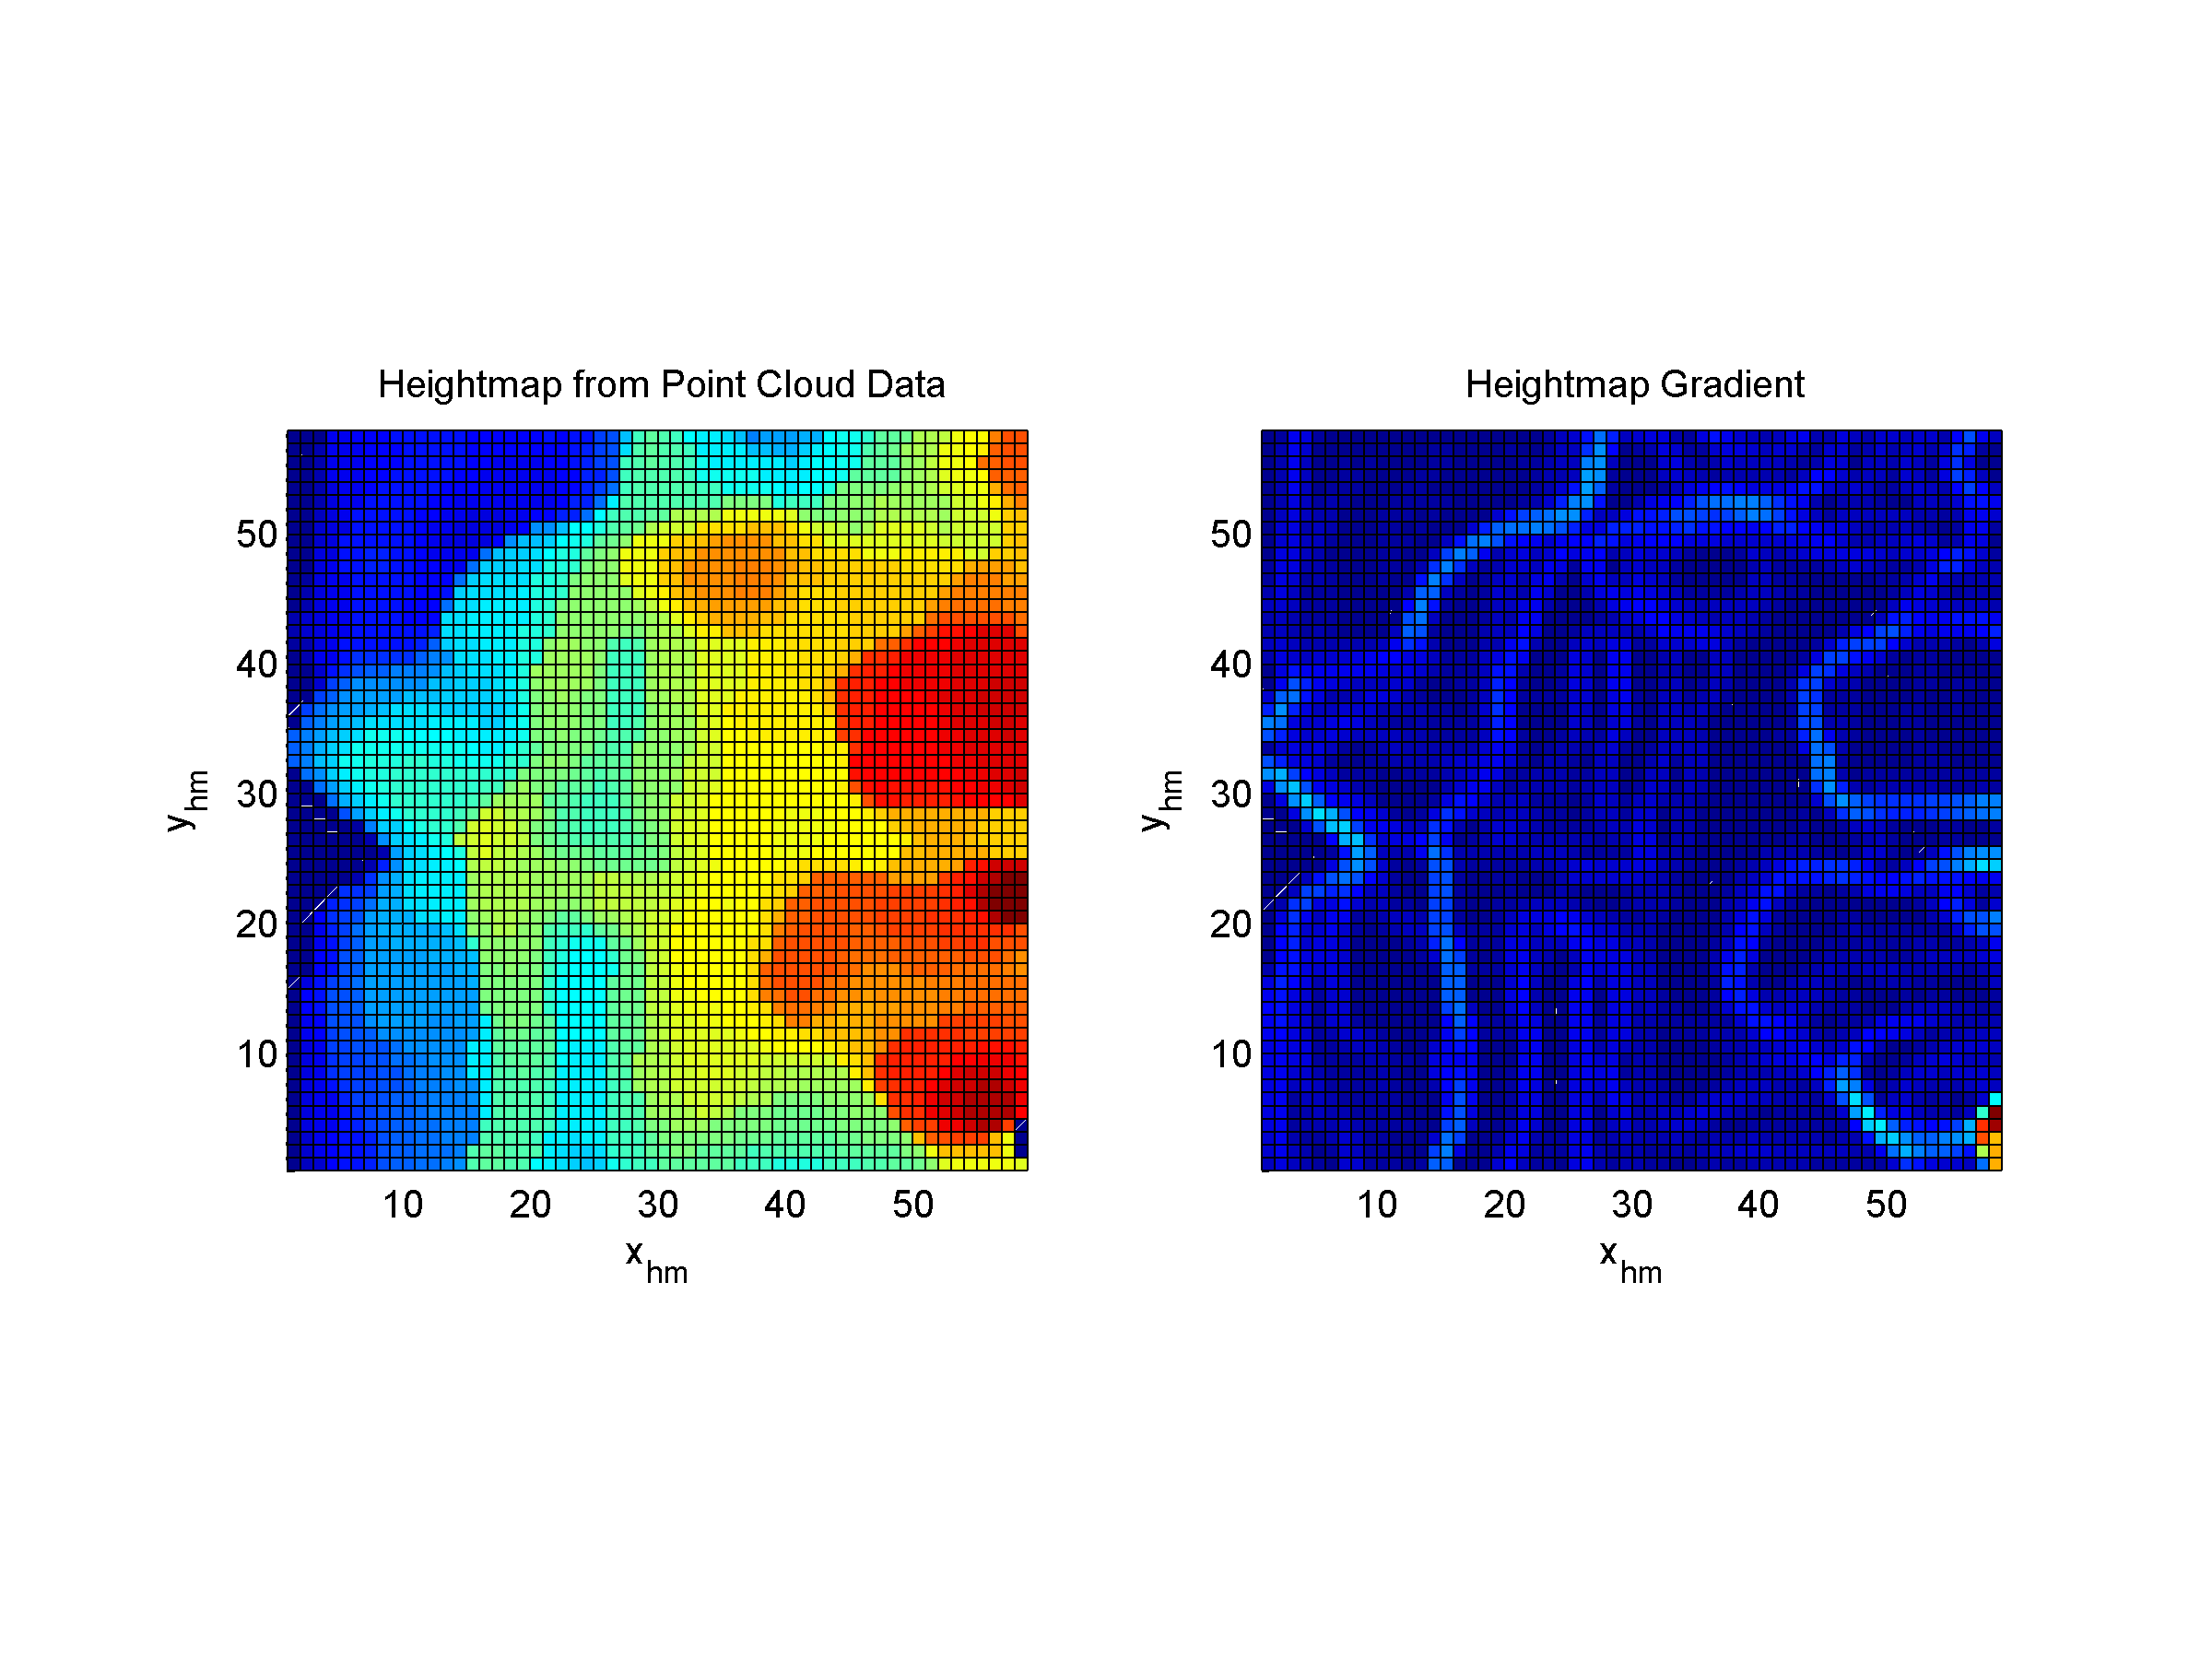
\includegraphics[width=\textwidth]{terrain_4545.png}}
					\caption{Height-map showing terrain variation in the $z_{hm}$ direction.}
					\label{fig::heightmap_terrain_patch_ortho}
				\end{figure}							
			The full 3D point cloud to height-map conversion is summarized in Algorithm \ref{alg::hmconvert}. In this algorithm, $\emph{\text{isolateROI}}$ is a function which locates a region of interest within the point cloud $\bar{S}$; $\emph{\text{getBestSubdivIndex}}$ performs the transformation in $\ref{eq::toheightmapframe}$, which generates indices within the discretized space $O_{Im}$ from points in $O_{0}$; $\emph{\text{dialateFeatures}}$ performs a standard image-dilation routine; and $\emph{\text{medianFilter}}$ performs a standard image median filter routine. Once a height-map has been generated, a corresponding gradient, as shown in \ref{fig::heightmap_terrain_patch}, is generated using a Sobel image gradient operation (from OpenCV).
			\begin{algorithm}[!h]
				\begin{algorithmic}
					\State{\textbf{init} $M = \Theta, w, d, \bar{S}$}
					\State{$\bar{S}_{ROI} = \text{isolateROI}(\bar{S})$}
					\ForAll{$\bar{x}_{k}\in \bar{S}_{ROI}$}
						\State{$[i,j] = \text{getBestSubdivIndex}(\xcomp{\bar{x}_{k}},\ycomp{\bar{x}_{k}},w,d)$}
						\If{$\zcomp{\bar{x}_{k}} > m_{i,j}$}
							\State{$m_{i,j} \leftarrow \zcomp{\bar{x}_{k}}$}
						\EndIf
					\EndFor
					\State{$M \leftarrow \text{dialateFeatures}(M)$}
					\State{$M \leftarrow \text{medianFilter}(M)$}
				\end{algorithmic}	
				\caption{3D ROI point cloud to height-map conversion.}
				\label{alg::hmconvert}
			\end{algorithm}

		\subsection{Generating a Cost-map from the Height-map}

			A discrete height-map space can easily be converted to a cost-space representation for the purpose of planning foot-placement during traversal over rough terrain. Here, a cost-map $C\in\Re^{n\times m\times l}$ is used in planning. The first and second dimensions of dimensions $C$ (of size $n$ and $m$) directly correspond to the width and depth of the discretized height-map space. The third dimension of size represents a discretization of the robot's yaw state, $\theta_{b,z}\in[-\pi,\pi]$ into $l$ subdivisions, and is used to represent variations of cost associated with each height-map indices, $[i,j]^{T}$, with respect to the robot's yaw. This cost map has been formulated with respect to three main cost elements:
				\begin{enumerate}
					\item variation in attainable foothold heights between all feet
					\item terrain steepness around any foothold, given a particular configuration
					\item net robot rotation performed at all step
				\end{enumerate}
			The first cost element is chosen to simplify to problem of ensuring the robot plans to walk over relatively level terrain by penalizing areas of the traversable terrain with larger variation in height. The second cost element is used deter the robot from attempting to travel over steep terrain. The final cost element is used to ensure the robot does not plan to perform any large changes in direction while traversing the terrain, which could cause for needless motion or loops in the planned path. 

			$C$ is used to generate an optimal, $K$-step path, which is comprised of $K$, discrete robot configurations. Moreover path is planned over rough terrain by optimizing a finite, $N$-step cost functional defined as follows:
				\begin{equation}			
					J(N) = \sum_{k=0}^N r_{c,k}
				\end{equation}	
			where  $r_{c,k} = r_{c}(\Gamma_{k},M,\nabla M)$. An optimal path can be found over the discretized space using an $A^{*}$-based path planning algorithm (or some variation). Additionally, sub-optimal paths could be generated using a potential fields approach. Both of these directions have yet to be explored as part of this project. Paths generated from the cost map would be mapped back into $O_{0}$ and interpolated to generate smooth trajectories.

			The function cost-map generation function $r_{c}(\Gamma_{k},M,\nabla M)$ represents a cost with respect to an immediate robot configuration, $\Gamma_{k}$, at the $k^{th}$ step of each planned trajectory; a height-map $M$; and its corresponding gradient $\nabla M$. The configuration parameter, $\Gamma_{k}$, is composed as follows:
				\begin{eqnarray}
					a_{k} 		&=& \ciel{l\wrap{\frac{\zcomp{\theta_{b,k}}+\pi}{2\pi}}} \nonumber\\
					\Gamma_{k} 	&=& \setwrap{p_{1,e,k}^{hm},...,p_{4,e,k}^{hm},a_{k}}
				\end{eqnarray}
			where $a_{k}\in\{0,...,l\}$ is an index which represent the discretized robot orientation parameter, $\theta_{b,k}$, at each \Kth step; and $p_{i,e,k}^{hm}$ represent the location of each \Ith within the height-map space (first two dimensions of the cost-space). The function $r_{c,k}$ is then defined as:
				\begin{equation}
					r_{c}(\Gamma_{k},M,\nabla M)
					= K_{v}\text{var}\wrap{h_{k}} 
					+ K_{g}\sum_{i=1}^{4}\wrap{\delta h_{i,k}^{2}} 
					+ K_{\theta}\wrap{\Delta a_{k}}^{2}
				\end{equation}
			where
				\begin{eqnarray*}
					h_{k} 			&=& \{h_{1,k},...,h_{4,k}\} \nonumber\\
					h_{i,k}			&\equiv& {m_{i_{i},j_{i}}}  \nonumber\\
					\delta h_{i,k}	&\equiv& {d_{i_{i},j_{i}}}  \nonumber\\
					\{i_{i},j_{i}\} &\equiv& \{ \wrap{p_{i,e,k}^{hm}}_{1}, \wrap{p_{i,e,k}^{hm}}_{2} \}
				\end{eqnarray*}
			$d_{i_{i},j_{i}}$ is the $(i_{i}^{th},j_{i}^{th})$ element of the height map gradient matrix, $\nabla M$; $K_{v},K_{g},K_{\theta}$ are weighting parameters.
%%
			





		\subsection{Surface Reconstruction}

			3D surface reconstruction is carried out according to a process for normal-estimation from 3D point cloud data detailed in \cite{Rusu2009}. According to this procedure, 3D surfaces are reconstructed from point cloud data, $\bar{S}$, by fitting a collection of flat polygonal elements to the source point cloud. Each of these estimated elements is represented by a surface-normal which emanates from a corresponding point within the source cloud. Surface normal estimation carried out by fitting planes to groups of points which exist within a neighborhood $d_{s}$ about each point $\bar{x_{i}}\in\bar{S}$.

			Before normal estimation, the point cloud $\bar{S}$ (which is usually dense) is down-sampled and smoothed before a normal estimation algorithm is applied. Point cloud down-sampling is performed using a voxel-grid technique, which discretizes the point cloud space into a voxel-space, which is a 3D space consisting of cuboids of a particular width, depth and height. Here, a cubic voxel space is used parameterized by a single voxel side-length dimension $d_{vox}$. The voxel grid filter and generates a single point from all points which fall within a voxel region, typically as a mean of all such points. The location of points which occupy the voxel region is aided by a KD-tree search technique, which offers higher efficiency over a brute-force search for neighboring points. This voxel-grid down-sampling technique produces a reduced representation of the original cloud, $\hat{S}$, which has shown, though observation of empirical results, to contain up to ten times less points, $\bar{S}$. This reduced-point cloud representation serves to greatly reduce the computation burden of successive cloud processing operations.

			Next, the resulting cloud, $\hat{S}$, is smoothed using a moving least-squares filter. This filter creates a smoothed point cloud by performing a sequence polynomial fits over subsets of points. As previously mentioned, normals are estimated from the smoothed point cloud via a plane fitting method, as described in \cite{Mitra2003}. Planes are estimated using Principle Component Analysis (PCA) on clusters of points \cite{Castillo2013}. The standard PCA algorithm provides a least-squares plane fit by way of dimensional reduction, yielding best-fit description for a set 3D points using a 2D manifold \cite{Pearson1901}. A point cloud with estimated surface normals is shown in Figure \ref{fig::surface_estimation}.
%%
			\begin{algorithm}[!h]
				\begin{algorithmic}
					\State{\textbf{init} $\bar{S},\bar{S}^{*},d_{vox},\vec{u}^{r},e,e_{max}$}
					\State{$\hat{S} = \text{voxelGridFilter}(\bar{S},d_{vox})$}
					\State{$\hat{S} \leftarrow \text{movingLeastSquaresFilter}(\hat{S})$}
					\State{$\hat{N} = \text{estimateNormals}(\hat{S})$}
					\ForAll{$\vec{n}_{i} \in N$}
						\State{$e = 1-(\vec{u}^{r})^{T} \vec{n}_{i}$}
						\If{$e<e_{max}$}
							\State{ $\bar{S}^{*} \leftarrow \bar{S}^{*} \cup \bar{x}_{i}$ }
						\EndIf
					\EndFor
				\end{algorithmic}	
				\caption{Finding good places to step from a 3D point cloud.}
				\label{alg::goodspacestostep}
			\end{algorithm}
%%
			Algorithm \ref{alg::goodspacestostep} is used to find ``flat" regions within the reconstructed surface for the purpose of footstep planning. Flat regions are located using generated surface, whose alignment is graded against a reference unit vector $\vec{u}^{r}$ by taking the dot product between  $\vec{u}^{r}$ and a surface normal to produce an alignment error $e\in[0,2]$. Points with associated normals whose alignment error is less than a scalar error bound, $e_{max}$, are selected as fit surfaces for walking. Obviously, not all surfaces which satisfy this alignment criteria represent surfaces which are fit for traversal. Post processing needs to be performed which segments the resulting point cloud clusters according their proximity to the robot.

			\begin{figure}[h!]
				\centering
				\fbox{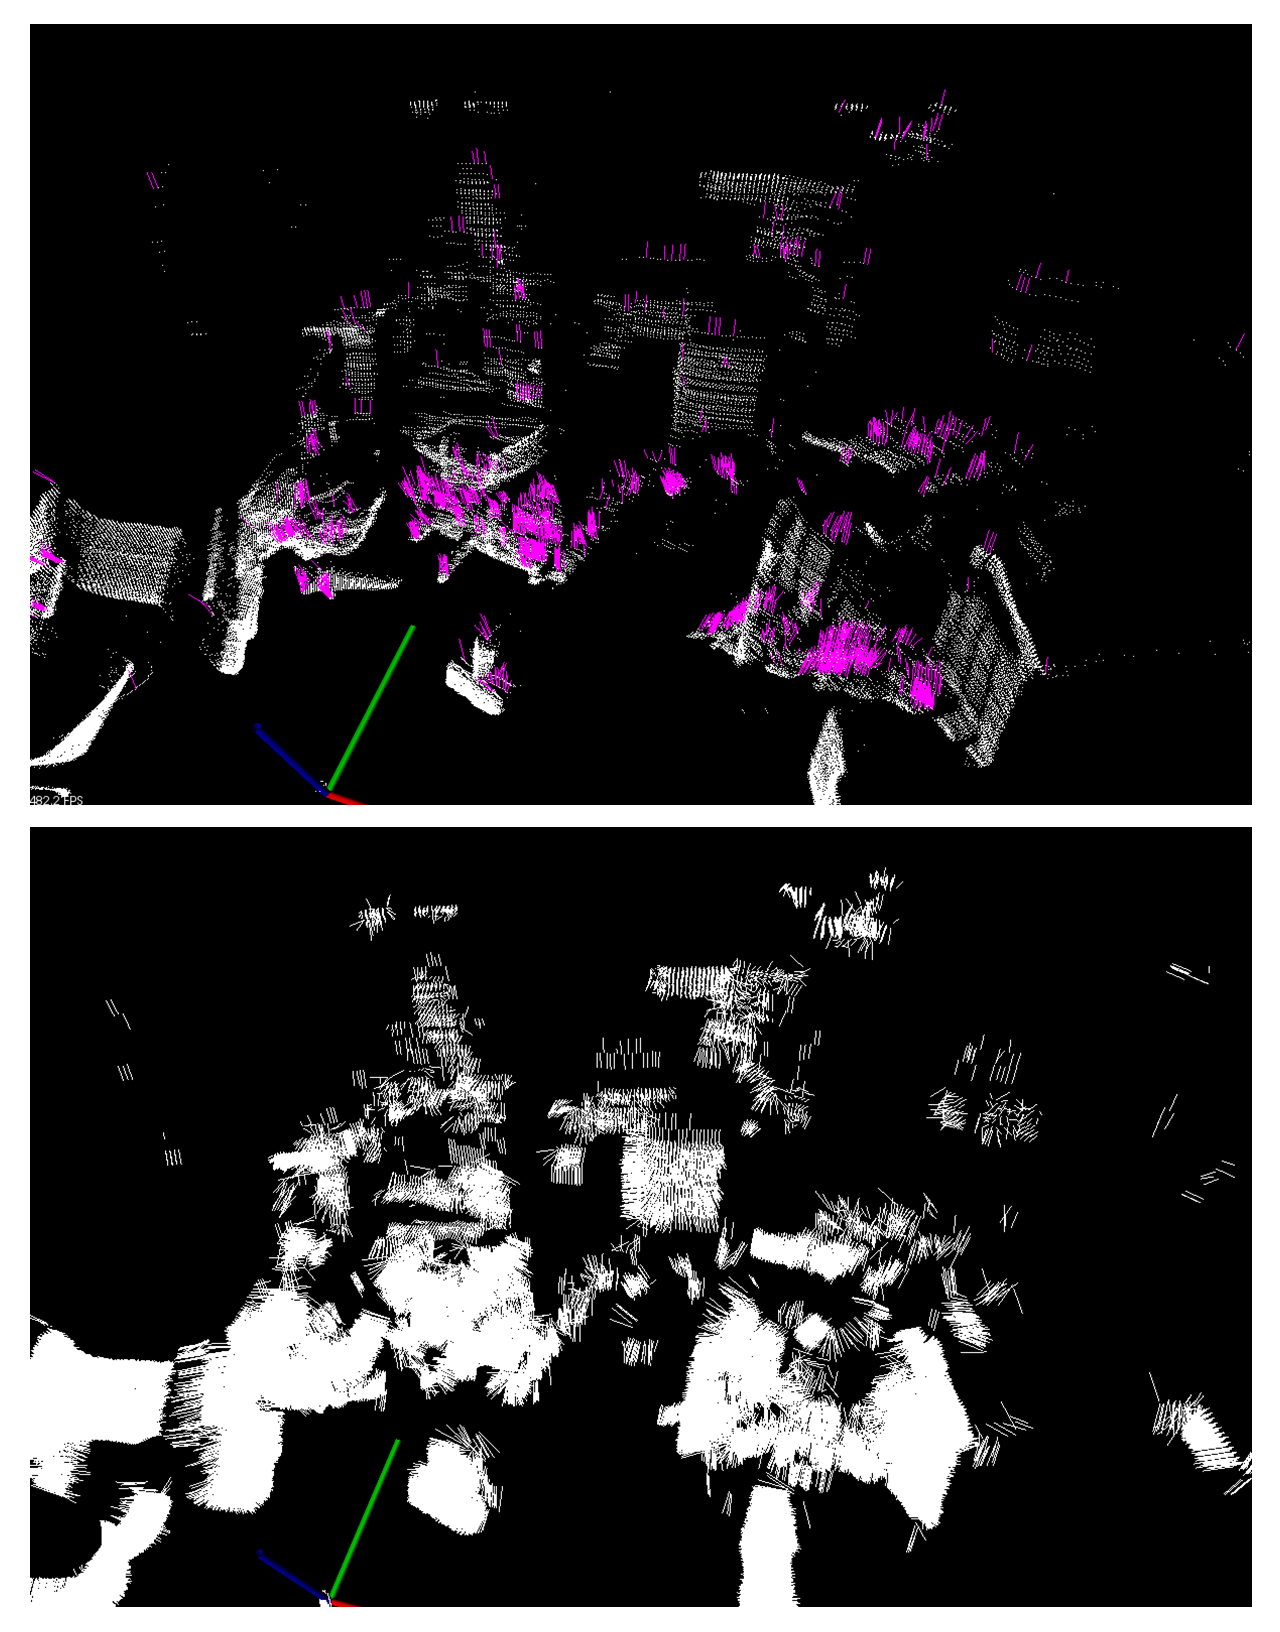
\includegraphics[width=\textwidth]{surf_reconstruction.png}}
				\caption{Point cloud generated from sequential scans of a room showing flat-surface candidates \emph{(top)} and 3D Point Cloud with normal estimation \emph{(bottom)}.}
				\label{fig::surface_estimation}
			\end{figure}